\documentclass[a4paper,14pt,cmcyralt]{report} %14-й шрифт
\usepackage[utf8]{inputenc}
\usepackage[T2A]{fontenc}
\usepackage[english,russian]{babel}
\usepackage{gnuplottex}
\usepackage{graphicx}
\graphicspath{{pics/}} %Папка для рисунков
\usepackage{amsmath,amssymb}
\usepackage{amsfonts}
\usepackage{textcomp}

\setcounter{tocdepth}{0}

\newcommand{\anonchapter}[1]{
\chapter*{#1}\addcontentsline{toc}{chapter}
{\numberline {}#1}
{\setcounter{section}{0}}
{\setcounter{figure}{0}}
{\setcounter{table}{0}}
{\setcounter{equation}{0}}
}

\newenvironment{introduction}

%\usepackage{geometry}
%\geometry{left=2cm}
%\geometry{right=2cm}
%\geometry{top=2cm}
%\geometry{bottom=2cm}

\begin{document}
\begin{titlepage}

\begin{center}
\MakeUppercase{Министерство образования и науки} \\
\MakeUppercase{Федеральное государственное автономное образовательное учреждение высшего образования} \\
«Национальный исследовательский технологический университет «МИСиС»

Институт новых материалов и нанотехнологий

\vspace{2cm}

ЛАБОРАТОРНЫЙ ПРАКТИКУМ

Физика конденсированного состояния

Электронные и оптические свойства твёрдых тел

\vspace{3cm}

авторы: \\
И.М. Анфимов \\
С.П. Кобелева \\
Л.Г. Спицина \\
И.В. Щемеров

\vspace{3cm}

МОСКВА, 2017 г.
\end{center}

\end{titlepage} %Титульный лист
\tableofcontents %Автоматический список литературы
\setcounter{chapter}{-1}
\chapter{Введение}

Предлагаемое учебное пособие предназначено для студентов института новых материалов и нанотехнологий (полупроводникового профиля) и преподавателей, проводящих лабораторные работы по курсу Физика конденсированного состояния, ч.1 <<Электронная структура твердых тел>>. В лабораторном практикуме рассматриваются методы измерения удельного электросопротивления, типа, концентрации и подвижности свободных носителей заряда. В теоретическом введении анализируются методы управления этими параметрами на основе зонной теории электронного строения кристаллических твердых тел и квантовой статистики.
\chapter{Измерение удельного электрического сопротивления полупроводников двухзондовым методом}

\section{Цель работы}
Определение распределения удельного электросопротивления по длине прямоугольного образца монокристаллического кремния двухзондовым методом при комнатной температуре.

\section{Теоретическое введение}
\subsection{Удельное электросопротивление}
\paragraph{Характеристика удельного сопротивления полупроводников}

Фундаментальным законом, устанавливающим связь между приложенным к проводящему образцу напряжением $U$ и протекающим в образце током $I$ является экспериментальный закон Ома:
\begin{equation}
I = \frac{U}{R}
\end{equation}
где $R$ - электросопротивление образца.

Электросопротивление $R$ зависит от геометрической формы и размеров образца, а также характеристики материала - удельного электросопротивления $\rho$. Для однородного образца правильной геометрической формы длиной $L$ и площадью поперечного сечения $S$
\begin{equation}
R = \rho \frac{L}{S}
\end{equation}

Если в этом случае выразить интегральные характеристики $I$ и $U$ через дифференциальные $j$ (плотность тока) и $\mathcal{E}$ (напряженность электрического поля), получаем закон Ома в дифференциальной форме
\begin{equation}
j = \frac{I}{S}, \mathcal{E} = \frac{U}{L} \rightarrow j = \frac{\mathcal{E}}{\rho} = \sigma \mathcal{E}
\end{equation}
где $\sigma$ - удельная электропроводность вещества.

В свою очередь, $\sigma$ определяется концентрацией свободных носителей заряда (СНЗ) $n$ и их подвижностью $\mu$:
\begin{equation}
\sigma = e n \mu
\label{UES}
\end{equation}

\begin{equation}
\mu = \frac{V_{\text{др}}}{\mathcal{E}}
\label{mu_from_Vdr}
\end{equation}
где $e = 1.6e^{-19}$ Кл - заряд электрона, $V_{\text{др}}$ - средняя дрейфовая скорость движения электрона под действием электрического поля.

Поведение $\sigma$ в кристаллических полупроводниках и металлах различно. Для металлов $\sigma$ - постоянная величина, в то время как в полупроводниках $\sigma$ зависит от примесного состава, кристаллического совершенства материала и внешних факторов — освещения, радиации и др. Эти материалы имеют также различный характер температурной зависимости удельной электропроводности.

Для полупроводников, у которых есть два типа СНЗ - электроны с концентрацией $n$ и дырки с концентрацией $p$ - формулу (\ref{UES}) необходимо дополнить:

\begin{equation}
\sigma = e n \mu_{n} + e p \mu_{p}
\end{equation}
где $\mu_{n}$ и $\mu_{p}$ - подвижность электронов и дырок соответственно.

\paragraph{Концентрация свободных носителей заряда}

Основой для понимания физических процессов и электрических явлений в твердом теле является зонная теория электронных спектров, базирующаяся на квантовомеханических представлениях. Концентрация свободных электронов — это концентрация занятых квантовомеханических состояний в зоне проводимости, а концентрация дырок — концентрация незаполненных состояний в валентной зоне. При температуре 0\textdegree К в полупроводнике свободных носителей заряда нет, в то время как концентрация электронов в металле практически не зависит от температуры и составляет величину порядка концентрации атомов металла в единице объема ($\approx 10^{22} \text{см}^{-3}$). СНЗ в полупроводниковых материалах появляются за счет термической генерации свободных носителей заряда (за счет энергии кристаллической решетки). Возможны несколько случаев:
\begin{enumerate}
\item переход электронов из валентной зоны в зону проводимости (в этом случае создаются одинаковые концентрации электронов и дырок $n = p = n_{i}$);
\item переход электронов из валентной зоны на уровень акцепторной примеси $E_{A}$, при этом создаются свободные дырки;
\item переход электронов с уровня донорной примеси $E_{\text{Д}}$ в зону проводимости (создаются свободные электроны).
\end{enumerate}

Верхний предел концентрации СНЗ при комнатной температуре в полупроводниках определяется пределом растворимости легирующих примесей ($\approx 10^{19} \text{см}^{-3}$), нижний предел определяется собственной концентрацией СНЗ - $n_{i}$.

Важнейшим параметром проводящего материала, однозначно связанным с концентрацией ННЗ, является уровень Ферми $F$. Для невырожденного материала
\begin{equation}
n = N_{c} \exp \left( -\frac{E_{c}-F}{k T} \right),
p = N_{v} \exp \left( -\frac{F - E_{v}}{k T} \right)
\end{equation}
где: $k$ – константа Больцмана, $N_{c}$ ($N_{v}$) — плотность состояний на дне зоны проводимости (потолке валентной зоны), зависящая от температуры и эффективной массы соответствующих СНЗ:
\begin{equation}
\begin{split}
%\begin{array}
N_{c} &= 2 \left( \frac{2 \pi m^{*}_{n} k T}{h^2} \right) = 4.82 \cdot 10^{15} \left( \frac{m^{*}_{n}}{m} \right)^{\frac{3}{2}} T^{\frac{3}{2}} = 2.5 \cdot 10^{19} \left( \frac{m^{*}_{n}}{m} \right)^{\frac{3}{2}} \left( \frac{T}{300} \right)^{\frac{3}{2}} \\
N_{v} &= 2 \left( \frac{2 \pi m^{*}_{p} k T}{h^2} \right) = 2.5 \cdot 10^{19} \left( \frac{m^{*}_{p}}{m} \right)^{\frac{3}{2}} \left( \frac{T}{300} \right)^{\frac{3}{2}}
%\end{array}
\end{split}
\end{equation}

Термодинамически равновесные концентрации $n$ и $p$ в невырожденном материале связаны соотношением:
\begin{equation}
n \cdot p = n_{i}^2 = N_{c} N_{v} \exp \left( -\frac{E_{g}}{2 k T} \right)
\end{equation}

При низких температурах доминирует процесс ионизации примеси, в области средних температур, к которой для большинства практически значимых полупроводниковых материалов относится комнатная температура, концентрация СНЗ равна концентрации легирующей примеси, и полупроводник является либо электронным, либо дырочным. При дальнейшем повышении температуры примесный полупроводник становится собственным. Температура перехода к собственной проводимости тем выше, чем больше ширина запрещенной зоны и чем выше концентрация легирующих примесей в полупроводнике.

Легирующими или мелкими примесями в полупроводнике, являются примеси, энергия ионизации которых ($E_{c}$ — $E_{\text{Д}}$ для донорной примеси и $E_{\text{А}}$ — $E_{\text{v}}$ для акцепторной) сравнима со средней энергией кристаллической решетки в расчете на один атом — $kT$ ($0.025$ эВ для комнатной температуры). Для широкого круга алмазоподобных полупроводников такими примесями являются элементы, валентность которых отличается от валентности атомов полупроводникового материала на единицу. Так, для кремния и германия легирующими будут элементы III (акцепторы) и V (доноры) групп периодической системы Менделеева. Для соединений $A_{III}B_{V}$ – элементы II и VI групп. Элементы IV группы в таких материалах могут быть как донорами, так и акцепторами, в зависимости от того, элемент какой из подрешеток они замещают.

\paragraph{Подвижность свободных носителей заряда}

Для объяснения того факта, что электрическое поле вызывает в проводящей среде движение с постоянной скоростью (\ref{mu_from_Vdr}), а не ускорением, как это должно быть при действии силы величиной $e \mathcal{E}$ на частицу с массой $m$, в классической теории электропроводности было введено понятие среднего времени свободного пробега $\tau$ как величины, обратной вероятности столкновения электрона с решеткой. При таком столкновении энергия, полученная от электрического поля, отдается решетки и восстанавливается первоначальный импульс. В этом случае подвижность определяется выражением:
\begin{equation}
\mu = \frac{\mathcal{E} \tau}{m}
\label{mu_from_E}
\end{equation}

В рамках классической физики было непонятно, почему длина свободного пробега $L$ (произведение времени свободного пробега на тепловую скорость носителя заряда) составляет сотни параметров кристаллической решетки, т. е. почему при движении по кристаллической решетке электрон сталкивается только с одним из сотен атомов на его пути. Объяснить этот экспериментальный факт (как и ряд других, связанных в частности, с различием поведения электропроводности металлов и полупроводников) удалось в рамках квантовомеханической теории, точнее, зонной теории кристаллических твердых тел. Электрон как квантовомеханическая ферми-частица обладает не только энергий и импульсом, но и волновыми свойствами. Волновая функция электрона в периодическом поле идеальной кристаллической решетки периодически модулирована с периодом, равным периоду обратной решётки, что позволяет электрону двигаться без рассеяния. В идеальном кристалле время свободного пробега и подвижность были бы бесконечными. Однако идеальных кристаллических решеток не существует в принципе. При взаимодействии с локальными нарушениями периодического Кулоновского поля, создаваемого ядрами атомов, т. е. с дефектами кристаллической решетки, импульс электрона изменяется. К основным дефектам кристаллической решетки можно отнести тепловые колебания атомов, примесные атомы (нейтральные и ионизированные), дислокации и т.д.

При приложении электрического поля изменяется заполнение разрешенных квантовомеханических состояний. При выключении за счет взаимодействия с дефектами решетки система релаксирует, переходя в термодинамически равновесное состояние. Поэтому вводится понятие времени релаксации, которое в слабых электрических полях совпадает с введенным в классической теории электропроводности понятием времени свободного пробега и связано с подвижностью СНЗ выражением (\ref{mu_from_E}).

Подвижность СНЗ зависит от среднего времени релаксации возбужденного состояния, которое, в свою очередь, определяется механизмом рассеяния СНЗ. Термин «механизм рассеяния» отражает тот факт, что в результате столкновения с дефектами кристаллической решетки поток электронов (дырок) вдоль направления вектора напряженности электрического поля постепенно уменьшается (рассеивается), что приводит к исчезновению электрического тока после выключения электрического поля. Но процессы рассеяния идут и при протекании электрического тока. Чем больше концентрация дефектов кристаллической решетки, тем быстрее происходит процесс выбывания отдельных электронов из потока, определяющего электрический ток в материале, тем меньше среднее время релаксации, подвижность СНЗ и величина электропроводности. Каждому типу дефекта кристаллической решетки соответствует свой механизм рассеяния.

Квантовомеханические расчеты показывают, что даже при 0\textdegree К атомы совершают колебания (нулевые колебания). С ростом температуры амплитуда колебаний растет, и растет вероятность столкновения электронов с колеблющимися атомами. Квазичастицы с характерным набором частот и волновых функций, с которыми эти колебания происходят, называются фононами, поэтому во всех кристаллах будет иметь место механизм рассеяния на фононах (тепловых колебаниях атомов кристаллической решетки). Любой дефект кристаллической решетки (нейтральные и ионизированные примесные атомы, дислокации, малоугловые границы и границы зерен и т.д.) вызывает появление соответствующего механизма рассеяния. В полупроводниках, помимо рассеяния на фононах, характерного для металлов, может доминировать рассеяние на ионизированных атомах примеси, а при низких температурах — на нейтральных примесных атомах. В целом в данном кристалле имеется столько различных механизмов рассеяния, сколько типов дефектов кристаллической решетки. С каждым из них связана свой величина подвижности $\mu_{i}$. Подвижность для (\ref{UES}, \ref{mu_from_Vdr}) определяется по формуле:
\begin{equation}
\frac{1}{\mu} = \sum\limits_{i = 1}^{N}{\frac{1}{\mu_{i}}}
\end{equation}
где $N$ - число типов дефектов.

Наибольший вклад в величину подвижности вносит тот механизм, значение подвижности для которого минимально. Он определяется доминирующим типом дефектов.

Отличие поведения полупроводников и металлов связано с тем, что в металлах электронный газ является вырожденным, а в полупроводниках - невырожденным. Последние описываются классической статистикой Больцмана. Относительно слабый линейный рост удельного электросопротивления металлов с температурой связан с уменьшением подвижности при рассеянии на длинноволновых акустических фононах, в то время как активационный рост этого параметра у полупроводников определяется температурной зависимостью концентрации СНЗ. Освещение не влияет на электропроводность металлов. В полупроводниках при освещении светом с энергией квантов, превышающей ширину запрещенной зоны, происходит переход электрона из валентной зоны в зону проводимости, что увеличивает электропроводность. Это явление называется фотопроводимостью. Поэтому при определении электропроводности полупроводников образец необходимо затенять. Это требование особенно важно для высокоомных материалов, в которых концентрация СНЗ мала.

При анализе электрофизических свойств в проводящих материалах чаще используется понятие удельного электросопротивления. В частности, марка наиболее распространенного полупроводникового материала — кремния — включает значение $\rho$ при температуре 23\textdegree С, выраженное в $\text{Ом}\cdot\text{см}$. Так, марка КЭФ-20 означает кремний электронный, легированный фосфором, с удельным электросопротивлением $20$ $\text{Ом}\cdot\text{см}$ при комнатной температуре, КДБ 4.5 — кремний дырочный, легированный бором, с удельным электросопротивлением $4.5$ $\text{Ом}\cdot\text{см}$ при комнатной температуре.

\subsection{Методика измерения удельного электросопротивления полупроводников}

Для измерения удельного сопротивления полупроводниковых образцов используются контактные и бесконтактные методы.
Зондовые методы осуществляют прямое измерение сопротивления определенной области образца по величине падения напряжения на ней при протекании определенного электрического тока (переменного или постоянного). Эти измерения основаны на законе Ома и производятся по двухзондовой, однозондовой (сопротивление растекания), четырехзондовой методикам.
Бесконтактные высокочастотные методы основаны на зависимости свойств скин-слоя характеризующего глубину проникновения высокочастотного (ВЧ) или сверхвысокочастотного (СВЧ) электрического поля в образец от величины его электропроводности. По способу подключения образца к ВЧ измерительному контуру различают емкостные методики (образец становится частью измерительного конденсатора) или индуктивные методики (образец помещается в катушку индуктивности). В СВЧ методе измеряется относительное изменение СВЧ мощности в СВЧ волноводе при взаимодействии образца с СВЧ волной. В отличие от зондовых методов эти методики неразрушающие, однако в виду сложности расчетов они являются не абсолютными, а эталонными, то есть определение электропроводности образца производится при сравнении с его эталонным образцом. Бесконтактные высокочастотные методы в отличие от зондовых методов могут измерять удельное сопротивление и поликристаллических образцов, так как влияние высокоомных межкристаллитных прослоек слабо сказывается в высокочастотных измерениях.

\section{Методика двухзондовых измерений удельного электросопротивления}

\subsection{Сущность двухзондового метода}

Двухзондовый метод измерения удельного электросопротивления требует применения монокристаллических образцов правильной геометрической формы (удлиненный прямоугольный параллелепипед или цилиндрический стержень) с нанесенными на торцевые поверхности образца омическими контактами. Из всех методов измерения он является наиболее точным, но и наиболее трудоемким. В производстве он применяется на заводах по выращиванию поликристаллического кремния на специально выращенных для определения параметров материала слитках. Схема двухзондового метода измерений представлена на рисунке \ref{1_base_scheme}.

\begin{figure}[h!]\centering
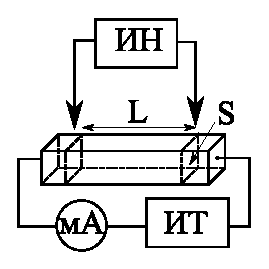
\includegraphics{pic1_1.eps}
\caption{Принципиальная схема двухзондового метода измерения удельного сопротивления: ИТ – источник тока; ИН – измеритель напряжения; $L$ – расстояние между зондами; $S$ – площадь сечения образца}
\label{1_base_scheme}
\end{figure}

Если по образцу протекает электрический ток силой $I$, создающий благодаря постоянству сечения образца одинаковую плотность тока в любой точке образца, то, измерив падение напряжения U между эквипотенциальными поверхностями, на которые установлены зонды, можно найти удельное сопротивление $\rho$ по формуле
\begin{equation}
\rho = \frac{U S}{I L}
\end{equation}

При этом предполагается, что эквипотенциальные поверхности перпендикулярны вектору плотности тока и сопротивлением контактов «зонд-полупроводник» можно пренебречь. Если первое условие при небольших сечениях образца удовлетворить легко, то второе условие, как правило, не удовлетворяется в силу особенностей контактных явлений между металлом и полупроводником.

Сопротивление образца на участке $x$ равно
\begin{equation}
R(x) = \int\limits_{0}^{x} {\frac{\rho(x)}{S} d x}
\end{equation}

Для однородного образца $\rho = const$ и $R(x) = \frac{d x}{S}$ - линейная функция от расстояния $x$. Если образец неоднороден, то зависимость $R(x)$ нелинейна, а сопротивление $\rho(x)$ можно найти по формулам

\begin{equation}
\begin{split}
\rho(x) &= S \cdot \tg(\phi) \\
\tg(\phi) &= \frac{d R}{d x} = \frac{\Delta R}{\Delta L}
\end{split}
\label{1_rho}
\end{equation}

\subsection{Анализ паразитных явлений и методика их устранения в двухзондовых измерениях удельного электросопротивления}

Пренебрежение влиянием контактных явлений может привести к грубым ошибкам измерения удельного сопротивления двухзондовым методом. Поэтому остановимся на описании вклада этих явлений подробнее.

\paragraph{Переходное сопротивление контакта «зонд-полупроводник».}
Из-за потенциального барьера (контактной разности потенциалов) вольтамперная характеристика (ВАХ) контакта металл-полупроводник является нелинейной, то есть сопротивление контакта зависит от величины и направления проходящего через него электрического тока. При измерении с помощью вольтметра падения напряжения между зондами в случае запирающих контактов, когда потенциальный барьер препятствует прохождению основных носителей заряда, один из контактов будет обладать высоким сопротивлением, которое может оказаться сопоставимым с внутренним сопротивлением вольтметра. Это внесет грубую ошибку в результат измерений. Избавиться от этой ошибки помогает компенсационный метод измерения падения напряжения, принципиальная схема которого представлена на рисунке \ref{1_potenc}. Для измерения падения напряжения используется потенциометр, представляющий собой калиброванный источник напряжения.

\begin{figure}[h!]\centering
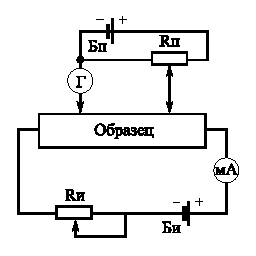
\includegraphics{pic1_2.eps}
\caption{Схема потенциометрического метода измерения}
\label{1_potenc}
\end{figure}

С помощью потенциометра $R_{\text{п}}$ между измерительными зондами создается компенсирующее напряжение $\text{Б}_{\text{п}}$, равное по величине и противоположное по знаку измеряемому. Последовательно с потенциометром в измерительную цепь включается чувствительный нуль-гальванометр Г. Если компенсирующее и измеряемое напряжение $\text{Б}_{\text{и}}$ равны по величине, то нуль-гальванометр фиксирует равенство нулю электрического тока, протекающего через измерительные зонды. В этом случае даже при высоком переходном сопротивлении контакта «зонд-полупроводник» падение напряжения на этом переходном сопротивлении равно нулю ($U_{\text{зонд}} = I R_{\text{зонд}} = 0$, т.к. $I = 0$).

Здесь следует добавить два важных замечания. Во-первых, внутреннее сопротивление потенциометра шунтирует сопротивление образца в цепи электрического тока, текущего через образец от источника тока, поэтом всегда должно соблюдаться требование $R_{\text{п}} \gg R_{\text{образца}}$. С учетом этого применяются для различных диапазонов измеряемых сопротивлений высокоомные потенциометры постоянного тока (ППТВ). Во-вторых, если нуль-гальванометр показывает равенство тока нулю, то это может означать, что протекающий ток меньше предела чувствительности гальванометра. Поэтому если использовать для измерения падения напряжения прибор, потребляющий электрический ток не выше предела чувствительности гальванометра, то он может заменить компенсационную схему измерения (то есть, обеспечить ту же погрешность измерения за счет вклада переходного сопротивления контактов).

\paragraph{Вклад паразитных термоЭДС.}

При измерении на высоких токах вдоль образца может возникать паразитная термоЭДС. Причиной появления термоЭДС является градиент температуры, возникающий при неравномерном разогреве образца за счёт протекающего тока. Знак этого градиента температуры не зависит от направления электрического тока. Благодаря этому такая термоЭДС может легко быть исключена из данных измерений при проведении двух измерений падения напряжения $U_{1}^{+}$ и $U_{2}^{-}$ между зондами при двух различных направлениях электрического тока. Падение напряжения на образце $U_{\text{обр}}$ и величину термоЭДС можно найти, определяя полусумму или полуразность величин $U_{1}^{+}$ и $U_{2}^{-}$ с учётом их знака.

\begin{equation}
\begin{split}
U_{1}^{+} &= I R_{\text{обр}} + U_{\text{ТЭДС}} \\
U_{2}^{-} &= -I R_{\text{обр}} + U_{\text{ТЭДС}} \\
U_{\text{обр}} &= I R_{\text{обр}} = \frac{U_{1}^{+} - U_{2}^{-}}{2} \\
U_{\text{ТЭДС}} &= \frac{U_{1}^{+} + U_{2}^{-}}{2}
\end{split}
\label{Uteds}
\end{equation}

Если токовые контакты не являются омическими, то при прохождении тока в них может возникать эффект Пельтье, то есть нагревание или охлаждение контакта в зависимости от направления тока. ТермоЭДС, создавшуюся в результате такого градиента температуры, вышеописанным способом устранить невозможно, так как она будет изменять знак с изменением направления тока. Неомичность токовых контактов также может привести к возникновению взаимосвязанных явлений инжекции, эксклюзии, экстракции и аккумуляции в приконтактных областях образца, которые могут изменить истинную величину электросопротивления. Следует делать минимальной величину тока, протекающего в образце, чтобы избежать разогрева образца, а также защищать образец от освещения во избежание возникновения в нем фотопроводимости или контактных фотоэдс. Все эти явления могут давать существенную погрешность измерения в высокоомных образцах.

\section{Описание измерительной установки}

Принципиальная электрическая схема установки показана на рисунке \ref{1_scheme}

\begin{figure}[h!]\centering
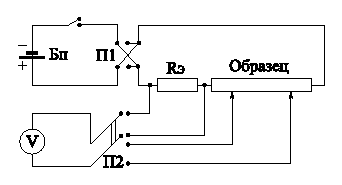
\includegraphics{pic1_3.eps}
\caption{Принципиальная схема измерений двухзондовым методом}
\label{1_scheme}
\end{figure}

Величина электрического тока через образец устанавливается при помощи управляемого линейного источника питания Б5-30. Точное определение тока производится по измерению падения напряжения $V$ на эталонном сопротивлении $R_{\text{э}}$, включённом последовательно с сопротивлением образца $R_{\text{обр}}$. Переключатель П2 может подключать вольтметр В7-21А или к образцу, или к эталонному сопротивлению. Переключатель П1 меняет направление электрического тока в образце. Источник тока может быть заменён батареей с подключённым последовательно переменным сопротивлением.

Исследуемый образец с нанесенным омическими контактами помещается в токовые зажимы на предметном столе в поле зрения оптического микроскопа. Определение расстояния между измерительными зондами производится с помощью микрометрической головки микроскопа. Нулевое положение устанавливается при совмещении перекрестия в поле зрения микроскопа с изображениями соприкасающихся первого и второго зондовых контактов. Полный оборот микрометрической головки микроскопа соответствует перемещению перекрестия на 1 мм.

Для определения типа проводимости образца применяется метод термозонда, принципиальная схема которого изображена на рисунке \ref{1_condtype}. Образец помещается на массивную металлическую пластину, служащую «холодным» контактом. Вместо массивного основания можно использовать холодный щуп. Нагретым с помощью небольшого электронагревателя зондом касаются верхней поверхности образца. Если образце имеет место проводимость n-типа, то электроны в образце диффундируют от нагреваемой термозондом верхней грани к «холодной» нижней грани, заряжая ее отрицательно. Верхняя грань образца будет заряжаться положительно за счет остающихся нескомпенсированными ионов донорной примеси $N_{D}^{+}$. Если образец имеет p-тип проводимости, то к «холодной» грани образца диффундируют положительно заряженные дырки, оставляя на «горячей» грани отрицательный заряд $N_{A}^{-}$ нескомпенсированных ионов акцепторов. Если в качестве регистрирующего устройства между горячим и холодным зондом включить параллельно светодиоды разного цвета, то при изменении типа проводимости измениться направление тока в цепи диодов и включится тот, напряжение на котором будет прямым. В используемом в работе детекторе в образце n-типа проводимости загорается зеленый светодиод, в образце p-типа — красный.

\begin{figure}[h!]\centering
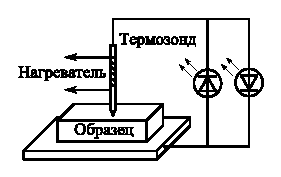
\includegraphics{pic1_4.eps}
\caption{Принципиальная схема измерений двухзондовым методом}
\label{1_condtype}
\end{figure}

\section{Порядок проведения работы и указания по технике безопасности}

\begin{enumerate}
\item Измерить толщину и ширину образца.
\item Установить образец на предметном столике и опустить на его поверхность измерительные зонды достаточно далеко от токовых контактов.
\item Установить необходимую величину тока через образец.
\item Привести в соприкосновение оба зонда, отметить нулевую точку отсчета на микрометрической головке микроскопа.
\item Повернуть микрометрическую головку микроскопа на 360\textdegree, переместить подвижный зонд на 1 мм по поверхности образца (конец зонда должен совместиться с перекрестьем в поле зрения микроскопа).
\item Измерить величину $U_{1}^{+}$ и $U_{2}^{–}$ с освещением и без освещения образца. Занести данные в таблицу \ref{1_table}.
\item Повторить п.п. 5 и 6.
\item Рассчитать зависимость $U_{\text{обр}}$ от расстояния $L$.
\item Изменить величину тока через образец и повторить измерение $U_{\text{обр}}$ от расстояния $L$.
\end{enumerate}

Электрический ток в измерительной схеме не превышает 3мА.

\section{Обработка результатов эксперимента}

\begin{enumerate}
\item Результаты измерений занести в таблицу \ref{1_table}, отметив условие освещённости образца.
\item Построить графики $R_{\text{обр}} = f(L)$ и $U_{\text{ТЭДС}} = f(L)$.
\item В соответствии с формулами (\ref{1_rho}) рассчитать $\rho(x)$.
\item Построить график $\rho(L)$ и сопоставить его с графиком $U_{\text{ТЭДС}}(L)$. Выполнить это построение для различных значений тока через образец и условий его освещенности.
\item Рассчитать погрешность измерения сопротивления Rобр и l и нанести их на графики.
\item Оценить погрешность определения удельного сопротивления $\delta \rho$.
\item Высказать суждение об однородности или неоднородности образца и влиянии величины электрического тока через образец и условий его освещенности на результаты измерений.
\end{enumerate}

\begin{table}[h]
\renewcommand{\arraystretch}{1.8} %% increase table row spacing
\caption{Измерение удельного электросопротивления при освещении (без освещения)}
\begin{center}
\begin{tabular}{c|c|c|c|c|c|c|c|c}
№ & $L$ & $U_{\text{э}}$ & $I = \frac{U_{\text{э}}}{R_{\text{э}}}$ & $U_{1}^{+}$ & $U_{2}^{-}$ & $U_{\text{обр}}$ & $U_{\text{ТЭДС}}$ & $R_{\text{обр}}$ \\
\hline
& мм & мВ & мА & мВ & мВ & мВ & мВ & Ом \\
\hline
\end{tabular}
\end{center}
\label{1_table}
\end{table}

\section{Контрольные вопросы}
\begin{enumerate}
\item Почему для определения удельной электропроводности полупроводниковых материалов применяют зондовые методы?
\item Достоинства и недостатки двухзондового метода измерения удельной электропроводности полупроводниковых материалов.
\item Как определить удельное сопротивление однородного и неоднородного образца при измерении двухзондовым методом?
\item Механизмы электропроводности в полупроводниках и металлах.
\item Какими факторами определяется величина концентрации свободных носителей заряда в полупроводниках и металлах при комнатной температуре?
\item Чем определяется температурная зависимость электропроводности полупроводников и металлов?
\item Какие процессы определяют появление свободных носителей заряда в области собственной и примесной проводимости?
\item От каких факторов зависит температура перехода от примесной проводимости к собственной?
\item Какие примеси создают n- или p- проводимость в полупроводнике?
\item Как влияет освещение на электропроводность полупроводников?
\item Какие материалы при измерении электропроводности необходимо затенять и почему?
\item Понятие механизма рассеяния свободных носителей заряда.
\item Назовите основные механизмы рассеяния свободных носителей заряда в полупроводниках и металлах.
\item В чем проявляется отличие свойств свободного электронного газа полупроводников и металлов?
\item Как влияет кристаллическое совершенство материала на электропроводность полупроводников и металлов?
\end{enumerate}

\section{Литература}
\begin{enumerate}
\item К.В. Шалимова. Физика полупроводников. СПб.: Лань, 2011 г.
\item В.В. Батавин, Ю.А. Концевой, Ю.В. Федорович. Измерение параметров полупроводниковых материалов и структур. М.: Радио и связь, 1985 г.
\item Л.П. Павлов. Методы определения основных параметров полупроводниковых материалов. М.: Высшая школа, 1975 г.
\item В.В. Горбачев, Л.Г. Спицина. Физика полупроводников и металлов. М.: Высшая школа, гл. 1, 1986 г.
\end{enumerate}
\newpage

\anonchapter{������������ ������ �2}
\setcounter{chapter}{2}

\begin{center}
����������� ������ ����������� ���� �������������� \\
(4 ����)
\end{center}

\section{���� ������}
����������� ������ ����������� ���� � �������-���������� ������ �� ������ ��������� ������������� ����������� ������������������.

\section{������������� �����}
\subsection{������������� ����������� ������������������}

����������� ���������, ���������� ������������� �� �������, �������� ���������� ������������������ ��������������� ��� ��������� �����������.

��� �������������� � ����� ���������� ����� ������������ �������� ������������������ ����� ����������� � ����:
\begin{equation}
\sigma = e n \mu
\end{equation}
��� $e$ - ����� ���������, $n$ - ������������ �������, $\mu$ - ����������� ��������� ������.

��� ������������ ������������������ � ������� � ������ ������ ���������, ���������� ��������� ������ ������� �� ���:
\begin{equation}
\sigma = e n \mu_{n} + e p \mu_{p}
\end{equation}

��� ������� ������������� ����������� �������������� ���������� ������� ����������� �� ����������� � ������������ ��������� ��������� ������ (���).

\subsection{������������� ����������� ����������� ���}

��� ������� ���������� ��������� ������������� n-����. �� ������� \ref{pic2_zone} �������� �������������� ��������� ��������� ��������������. ����� ��� ����������� ������������ �� ����������� ��� �������������� �������������� � ����� ����� �������� ������� ����������� �� ������� \ref{pic2_n_T}.

\begin{figure}[h!]\centering
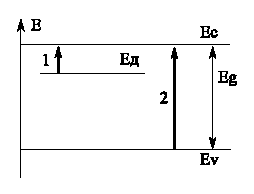
\includegraphics[height=4cm]{pic2_zone.eps}
\caption{������ ��������� � ����� ����� �������� �������}
\label{pic2_zone}
\end{figure}

\begin{figure}[h!]\centering
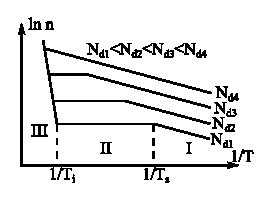
\includegraphics[height=4cm]{pic2_n_T.eps}
\caption{����� ��� ������������� ����������� ������������ ��� �������������� �������������� � ����� ����� �������}
\label{pic2_n_T}
\end{figure}

�� ����������� $\ln n = f(\frac{1}{T})$ ����� �������� ��� ����������� ������������� ���������.

\paragraph{I. ������� ��������� ���������.}
��� ���������� ���� ��������� ���� �������������� ������� ��������� �����������. � ���� ������������ ��� ��������� ���������. ��� ��������� ����������� ��������� ��������� � ������� �������� ������� � ���� ������������, ������������ ��������� ���������� ����������. ��� ������� ���������� ���������� ������ ������� � ������������ ������ �� ����������� ��������� ������� $T = T_{s}$. � ���� �������
\begin{equation}
n = \sqrt{\frac{N_{c}N_{d}}{2}} \exp{\left( -\frac{E_{d}}{2 k T} \right)}
\label{eq2_n_T}
\end{equation}
��� $N_{c} = 2 \left( \frac{2 \pi m_{dn}^{*} k T}{h^2} \right) ^ \frac{3}{2}$ - ����������� ��������� ��������� � ���� ������������, $E_{d}$ - ������� ��������� �������� �������, $N_{d}$ - ������������ �������.

\paragraph{II. ������� ��������� �������.}
� ������� ���������� $T_{s} < T < T_{i}$ �������� ������� ��������� ����������, �� ����������� ��������� ��� �� ��������. ������� ������������ ��������� ���������� ��������� � ����� $N_{d}$.
������ ������� ��������� ������� �� ������������ ������������ ������� � � ������� ���������. ��� ���������� ���� ������� ������������� �������� ������� ��������� ����� �����������. ��� ���������� ������� ��������� $N_{d}$ �� ����� ��������� ���������.

\paragraph{III. ������� ����������� ���������.}
� ������� ������� ���������� $(T > T_{i})$, ����� ������� ��������� �������� ���������� ���������� ������������ � ������� ����������� ���� $(k T \approx E_{g})$, ��������� �������� ���������� �� ��������� ���� � ���� ������������, ��-�� ���� ������������ ��������� ��������� ����� ����������. ���������� ��������� ������ ��������� �������.

\begin{equation}
n_{i} = \sqrt{N_{c} N_{v}} \exp{\left( -\frac{E_{g}}{k T} \right)} \sim T^{\frac{3}{2}} \exp{\left( -\frac{E_{g}}{k T} \right)}
\label{eq2_ni_T}
\end{equation}

������ ����������� ���� ����� ������� �� �����������. ��� ����������� ��������������� �������� $E_{g}$ ������� ������� ��������� � ������������, ������ � ������� ��������� ���������� ��� ����� ���� ���������������� ������ ������:
\begin{equation}
E_{g}(T) = E_{g}(0) + \alpha T
\label{eq2_E_T}
\end{equation}
��� $E_{g}(0)$ - ��������, ������� ����� �������� �������������� ������������� ����������� ������ ����������� ���� �� �������� 0\textdegree �, $\alpha$ - ������������� ����������� ��������� ������ ����������� ����, ������ ����������� � ���������� ������� ���� ���/�.

�� ������� \ref{pic2_E_T} �������� ������������� ����������� ������ ����������� ���� � �������.

\begin{figure}[h!]\centering
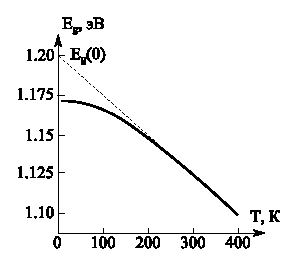
\includegraphics[height=4cm]{pic2_E_T.eps}
\caption{������������� ����������� ������ ����������� ���� ��� �������}
\label{pic2_E_T}
\end{figure}

���������� (\ref{eq2_E_T}) � (\ref{eq2_ni_T}) ��������:
\begin{equation}
n_{i} = \sqrt{N_{c} N_{v}} \exp{\left( -\frac{E_{g}(0) + \alpha T}{k T} \right)} \sim T^{\frac{3}{2}} \exp{\left( -\frac{E_{g}(0)}{k T} \right)} \exp{\left( -\frac{\alpha}{k} \right)}
\label{eq2_ni_T}
\end{equation}

\subsection{������������� ����������� ����������� ���}
����������� ����� ������� �� �����������. �������� ����������� ������������ ������������ ���������� ��������� � �������������� ��� ������ �����������. ��� ����������� ���������� ����������� $\mu(T)$ ����� ���� ���������� ��������� �����������:
\begin{equation}
\mu(T) = \mu_{i} \left( \frac{T}{T_{i}} \right)^{m}
\end{equation}
��� $\mu_{i}$ - ����������� ��� ����������� $T = T_{i}$.

���� �������� ���������� �������� ��������� �� ����� �������, ���������� $m = \frac{3}{2}$. ��� ��������� �� ����������� �������� $m = 0$, � ��� ��������� �� ������������ ������� $m = -\frac{3}{2}$. � �������� ��������������� ������������ ��������� ��������� ���������� ���������, ������� ����������� �������� ���������� $m$ ����� ��������� ������ ��� ������������� ��������� ����������. ��� ���� ��������� ���������� ��������� - �� ������������ ������� � ����� ������� - ������������� ���������� ����������� ��������� ���, ���������� �� ������� \ref{pic2_mu_T}

\begin{figure}[h!]\centering
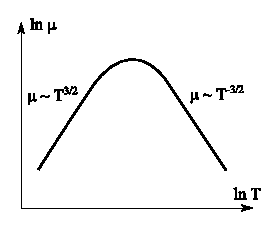
\includegraphics[height=4cm]{pic2_mu_T.eps}
\caption{������������� ����������� ����������� ��������� ��������� ������ � ������������� ��������������}
\label{pic2_mu_T}
\end{figure}

� ������� ������ ���������� ������������ ���������� ��������� �������� ��������� �� ����� �������. � ������ ����������� ����������� �������������, ��� ��� ������������� �������� �������� ���������, � ��� �������������� � ������������� �������� (��������� ������) �������� ����������� �� ������� ����. � ���������� ������ ����������� ������� ���������� ��������� �������� ��������� ������� �������, � ����������� �������������� ���������� �� ������������ �������, �������. ��� ���� ����� � �������� ��������������� ���������� ����������� ��� ������ ������ ����� ���������� �� ���������� �������� $m = -\frac{3}{2}$ � ������� ���� � �� ��� ������ �������.

� ������ ������ (\ref{eq2_n_T}) � (\ref{eq2_ni_T}) ����� ��������� ����������� ������������������ �� �����������. ��������� ��� ����� ����������� ������� �� ������� \ref{pic2_sigma_T}.

\begin{figure}[h!]\centering
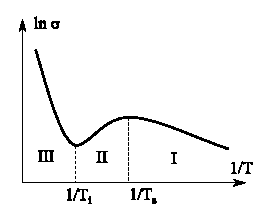
\includegraphics[height=4cm]{pic2_sigma_T.eps}
\caption{������������� ����������� ������������������ � ������������� ��������������}
\label{pic2_sigma_T}
\end{figure}

�� ���������� ������� ����� �������� ��� �������.

I. ������� ��������� ������������
\begin{equation}
\sigma = e n(T) \mu(T) \sim T^{\frac{3}{4} + m} \exp{\left( -\frac{E_{d}}{2 k T} \right)}
\end{equation}

II. ������� ��������� �������
\begin{equation}
\sigma = e N_{d} \mu(T) \sim N^{m}
\end{equation}

III. ������� ����������� ������������
\begin{equation}
\sigma_{i} = e n_{i}(T) \left[ \mu_{n}(T) + \mu_{p}(T) \right] \sim T^{\frac{3}{2} + m} \exp{\left( -\frac{\alpha}{2 k} \right)} \exp{\left( -\frac{E_{g}(0)}{2 k T} \right)}
\end{equation}

� ���������� ����������� ���� ��������� ����������� ������������. � ������� ��������� ������� ������������� ����������� ������������������ ������������ ������������� ������������ �����������. � �������� ��������� � ����������� ��������� ������� ������� ��������� ������������� ����������� ������������ ���������.

���� ���������� ������ ��������� ����������� ������ ����������� ���� �� �����������, �� ������� (I) � (III) ����� ��� ������ � ��������� ���� ������� $-\frac{E_{d}}{2 k T}$ � $-\frac{E_{g}(0)}{2 k T}$ ��������������. ����� �������, ����������������� ����������� ��������� ������������ �� �������� ����������� ��������� ���������� ������� ��������� � ������ ����������� ���� �����������������. ��� ���� ����� �������, ��� �������� $E_{g}(0)$ �� ����� � �������� ������ ����������� ���� � �������������� ��� ����������� 0\textdegree �, � �������� ������, � ������� �������� ������������� ����������� ��� ������� ���������� ���������� ��� �������. ������ ��� ����������� $E_{g}$ �� ����� ������������� ����� ��������� ������ ���������.

\section{�������� ��������� � �������� ���������}

� ������ ������ ������������ �����, ���������� �� ������� \ref{pic2_scheme}. ������� $R_{\text{���}}$ ���������� � ���� ��������������� � �������� - ������� �������������� ������� ��������� �������� $R_{\text{���}}$. � ���� ��������� ����� ���� ������������ ���, ��� ���� ������� ���������� �� $R_{\text{���}}$ � $R_{\text{���}}$ ��������� ��� ������ �������������� ������ Fractal MCX 52.1. �������� ���� ����� ������� $I_{\text{���}}$ ����� ���� ����� ��������� ������������� � ����� ���� ������� ���
\begin{equation}
I_{\text{���}} = I_{\text{���}} = \frac{U_{\text{���}}}{R_{\text{���}}}
\end{equation}

\begin{figure}[h!]\centering
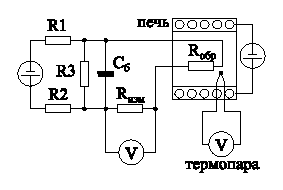
\includegraphics[height=4cm]{pic2_scheme.eps}
\caption{�������������� ����� ��������� ��� ��������� ������������� ����������� ��������������������}
\label{pic2_scheme}
\end{figure}

��� ��� ���������� ���������������� �����-������ ��� � ������� ������ MCX ��������� � ��������� �� $0.02$ �� $2.56$ �, �� � ����� ������������ �������� ����������, ����������� �� ���������� $R1$, $R2$ � $R3$.

����� ��������� ������� ��������, ������� ����� ���������� ��-�� ��������� ����������� ����� �������, ��������� ������������ ��������� ���������� � ���� ������������. ����������� $C_{\text{�}}$ ���������� ����������� ���������, �������� ������� ����.

������� � ����������� ��������� ���������� � ��������� ������ �����������, ������� �������� �������������� �� ��������� �378. ����������� ������� ���������� ����������, ������ � ������� ������������� ��������������� ������������� ������� MCX 52. ���������� ��������� ������� ���������� �� �������, ��������� ������������� � ������ � ��������� ��������������� ���������� ��� � ���������� �� ���������, ��� �� ���������� � ������ ���������� � ������������� ������ ��������������� � ������������� ����������� ������� � �����������.

\section{������� ���������� ������ � �������� �� ������� ������������}

\begin{enumerate}
\item ��������� ��������� ��� ��������� ������������� ����������� ��������������������.
\item ���������� ����� <<���������>> � ������� ������������ � ������ ������ COM-port.
\item ��������� ��������� � �������� ������, ����� 50� �� �����������.
\item ������� ������� �� 120\textdegree C.
\item ��������� ������, �������� ������� �� 40\textdegree C.
\item ��������� ���������� ���������.
\end{enumerate}

����� ������� ��������� ���������� ��������� � ���, ��� �������� ����� � �������� ��������� ���������. ��� ������ � ����� ����������� ��������� ����������� ���� 200\textdegree C.

\section{��������� ����������� ������������}

\begin{enumerate}
\item ���������� ��������� ������� � �������, ������� ������� ������� � ����������.
\item ���������� �������� ��������� � ����������� $\ln \sigma = f \left( \frac{1}{T} \right)$.
\item �� ���������� ������� (��������� ��� ������� �� ������� \ref{pic2_experiment}) �������� ��� �������� �������, ����� ������������� ����������� ������������, ������ - ���������.
\item ������ ������ ������������ ��������� ������� ���������. � ������� ����������� ������������ $\tg (\phi_{2}) = -\frac{E_{g}(0)}{2 k}$, ������ $E_{g}(0) = -2 k \tg(\phi_{2})$.
\item ���������� ���������� ������� ��������� ������� $E_{d} = -2 k \tg(\phi_{1})$.\
\item ���������� ������ ���������, ��������� ������� ��������� �� ��������� �������� ������.
\end{enumerate}

\begin{table}[h!]
\caption{��������� ��������� �������������������� ��� ��������� (��� ���������)}
\begin{center}
\begin{tabular}{c|c|c|c|c|c|c|c}
� & $U$ & $t$ & $T$ & $R$ & $\sigma$ & $\ln(\sigma)$ & $\frac{1}{T}$ \\
\hline
& �� & \textdegree C & � & �� & $\text{��}^{-1} \text{��}^{-1}$ &  & K \\
\hline
\end{tabular}
\end{center}
\end{table}

\begin{figure}[h!]\centering
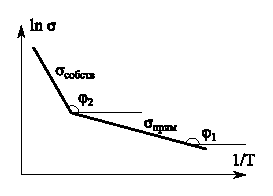
\includegraphics[height=4cm]{pic2_experiment.eps}
\caption{�������� ��� ������������� ����������� ������������������ ��������������}
\label{pic2_experiment}
\end{figure}

\section{����������� �������}

\begin{enumerate}
\item ������� ������ ����������� ���� � ������� ��������� �������.
\item ������������� ����������� ������ ����������� ���� � ���������������.
\item ������������� ����������� ������������ ��������� ��� �������������� �������������� � ���� ���������� ����� ������������.
\item ��������� ��������� ��������� ������ � ���������������.
\item ������������� ����������� ����������� ��������� ����� � ���������������.
\item ������������� ����������� ������������������ � ���������������.
\item ����������� ������� ��������� ������� �� ������������� ����������� ��������������������.
\item �������� �������, ������������� �������� ���������.
\end{enumerate}

\section{����������}

\begin{enumerate}
\item �.�. ������. ����� ��������������. �.: ������ �����, 1975.
\item �.�. ��������, �.�. �������. ������ ��������������� � ��������. �.: ������ �����, ��. 3, 1986 �.
\item �.�. ������. ������ ����������� �������� ���������� ����������������� ����������. �.: ������ �����, 1975 �.
\end{enumerate}
\newpage

\anonchapter{Лабораторная работа №3}
\setcounter{chapter}{3}
\setcounter{section}{0}
\setcounter{figure}{0}
\setcounter{table}{0}
\setcounter{equation}{0}

\begin{center}
Определение подвижности основных носителей заряда \\
(4 часа)
\end{center}

\section{Цель работы}
Определение подвижности основных носителей заряда в полупроводнике и коэффициента Холла по измерениям эффекта холла.

\section{Теоретическая часть}

\subsection{Возникновение поля Холла}

Эффект Холла заключается в возникновении поперечного электрического поля в образце, через который протекает электрический ток, помещённом в магнитное поле, перпендикулярное направлению этого тока. Если в магнитном поле с индукцией $\overrightarrow{B}$ находится полупроводник n-типа, по которому течёт ток плотностью $\overrightarrow{j}$, то на электроны, движущиеся со скоростью $\overrightarrow{v}$ будет действовать сила Лоренца, отклоняющая их в сторону. Таким образом, на одной из граней появится отрицательный заряд, а на другом начнут скапливаться нескомпенсированные доноры. В дырочном полупроводнике механизм останется тем же, но знаки зарядов и направление их движения изменятся (см. рисунок \ref{pic3_lorentz}).

\begin{figure}[h!]\centering
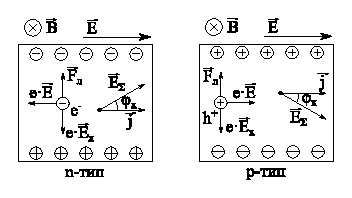
\includegraphics[height=4cm]{pic3_lorentz.eps}
\caption{Проявление эффекта Холла в образцах n- и p-типа проводимости.}
\label{pic3_lorentz}
\end{figure}

Возникающие на гранях, параллельных течению тока и индукции магнитного поля, заряды, создают электрическое поле $\overrightarrow{E}_{\text{х}}$, стремящееся компенсировать отклонение зарядов под действием силы Лоренца. Суммарное поле $\overrightarrow{E}_{\Sigma}$ будет направлено под углом $\phi$ к току, направление которого не изменится. Напряжённость поля $\overrightarrow{E}_{\text{х}}$ пропорциональна векторному произведению $\overrightarrow{B}$ и $\overrightarrow{j}$ с коэффициентом пропорциональности $R_{\text{х}}$.

\begin{equation}
\overrightarrow{E}_{\text{х}} = \overrightarrow{R}_{\text{х}} \left[ \overrightarrow{B} \times \overrightarrow{j} \right]
\label{eq3_vector_lorentz}
\end{equation}

$R_{\text{х}}$ называется коэффииентом Холла, а $\phi$ - углом Холла.

Как видно из рисунка \ref{pic3_lorentz}, направление силы Лоренца не зависит от знака заряда, а значит по направлению поля Холла можно определить тип основных носителей заряда в полупроводнике. Коэффициент Холла отрицателен в полупроводнике n-типа, и положителен для p-типа.

\subsection{Определение коэффициента Холла}

Если все углы между $\overrightarrow{B}$, $\overrightarrow{j}$ и $\overrightarrow{E}_{\text{х}}$ прямые, и не учитывается распределение электронов по скоростям, то (\ref{eq3_vector_lorentz}) можно переписать как

\begin{equation}
E^{y}_{\text{х}} = \frac{1}{e n} j^{x} B^{z}
\end{equation}
где $e$ - заряд электрона, $n$ - концентрация свободных носителей заряда.

В таком случае $R_{\text{х}} = \frac{1}{e n}$. Для учёта различия между полной скоростью электронов, входящей в выражение для силы Лоренца, и дрейфовой скоростью, которую электрон принимает под действием поля, а также распределения электронов по скоростям, решается кинетическое уравнение Больцмана. Точное решение приводит к необходимости введения коэффициента $r_{\text{х}} = \frac{<\tau^{2}>}{<\tau>^2}$, называемого холл-фактором, $\tau$ - время релаксации при данном основном механизме рассеяния.. В таком случае полное выражение для коэффициента Холла выглядит следующим образом:

\begin{equation}
R_{\text{х}} = \frac{r_{\text{х}}}{e n}
\end{equation}

Расчёты показывают, что для невырожденных полупроводников при рассеянии на акустических фононах $r_{\text{х}} = \frac{3}{8} \pi$, а при рассеянии на ионах примеси $r_{\text{х}} = \frac{315}{512} \pi$. Для вырожденных полупроводников и металлов величина $r_{\text{х}}$ от доминирующего механизма рассеяния не зависит и равна единице. Для сильных магнитных полей ($\mu B \gg 1$) коэффициент Холла не зависит от механизма рассеяния и степени вырождения, а определяется только концентрацией носителей заряда: $R_{\text{х}} = \frac{1}{e n}$.

В случае смешанной проводимости и в материалах близких к собственным коэффициент Холла опреедляется следующим соотношением:
\begin{equation}
R_{\text{х}} = \frac{r_{\text{х}}}{e} \frac{p \mu_{p}^{2} - n \mu_{n}^{2}}{\left( p \mu_{p} + n \mu_{n} \right)^{2}}
\end{equation}

В области примесной проводимости по коэффициенту Холла и электропроводности можно определить концентрацию основных носителей заряда, а по тангенсу угла Холла - их подвижность.

\subsection{Методика измерения и описание установки}

В ходе данной работы через образец, имеющий форму прямоугольного параллелепипеда, пропускается постоянный ток, и измеряется разность потенциалов, возникающая на холловских контактах (см. рисунок \ref{pic3_sample}). В данном случае

\begin{equation}
\begin{split}
V_{\text{х}} &= b E_{\text{х}} \\
V &= a E \\
I &= b d j
\end{split}
\end{equation}

\begin{figure}[h!]\centering
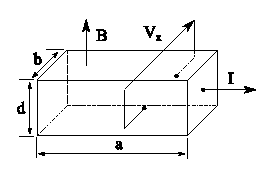
\includegraphics[height=4cm]{pic3_sample.eps}
\caption{Линейные размеры образца и расположение основных векторов}
\label{pic3_sample}
\end{figure}

Эти формулы можно переписать в виде:
\begin{equation}
\begin{split}
V_{\text{х}} &= - \frac{R_{\text{х}} I B}{d} \\
V &= \frac{I}{\sigma} \frac{c}{b d}
\end{split}
\end{equation}

Угол между направлением электрического поля в образце и полем Холла называется углом Холла и определяется как:
\begin{equation}
\tg \phi = \frac{E_{\text{х}}}{E} = \frac{a}{b} \frac{V_{\text{х}}}{V}
\label{eq3_tg}
\end{equation}

Измерив падение напряжения в продольном и поперечном направлении, а также индукцию магнитного поля, можно рассчитать основные характеристики образца:
\begin{equation}
\begin{split}
\sigma &= \frac{c}{b d} \frac{I}{V} \\
R_{\text{х}} &= d \frac{V_{\text{х}}}{I} \frac{1}{B} \\
\mu_{\text{х}} &= \frac{c}{b} \frac{V_{\text{х}}}{V} \frac{1}{B}
\end{split}
\label{eq3_mu}
\end{equation}

На точность измерения эффекта Холла влияет геометрия образца. Поперечное напряжение можно считать равным ЭДС Холла только при отношении длины образца к ширине не менее $3:1$.

Для измерения коэффициента Холла применяется стандартный метод постоянного тока и постоянного магнитного поля. Уменьшение вклада паразитных эффектов производится усреднением результатов измерения при разных направлениях тока и индукции. Пусть

\begin{equation}
\begin{split}
V_{I^{+}B^{+}} &= V_{\text{х}} + V_{\text{асм}} + V_{\text{мр}} + V_{\text{ТЭДС}} + V_{\text{Э}} + V_{\text{НЭ}} + V_{\text{ПНЭ}} + V_{\text{РЛ}} + V_{\text{ПРЛ}} \\
V_{I^{-}B^{+}} &= -V_{\text{х}} - V_{\text{асм}} - V_{\text{мр}} + V_{\text{ТЭДС}} - V_{\text{Э}} + V_{\text{НЭ}} - V_{\text{ПНЭ}} + V_{\text{РЛ}} - V_{\text{ПРЛ}} \\
V_{I^{-}B^{-}} &= V_{\text{х}} - V_{\text{асм}} - V_{\text{мр}} + V_{\text{ТЭДС}} + V_{\text{Э}} - V_{\text{НЭ}} + V_{\text{ПНЭ}} - V_{\text{РЛ}} + V_{\text{ПРЛ}} \\
V_{I^{+}B^{-}} &= -V_{\text{х}} + V_{\text{асм}} + V_{\text{мр}} + V_{\text{ТЭДС}} - V_{\text{Э}} - V_{\text{НЭ}} - V_{\text{ПНЭ}} - V_{\text{РЛ}} - V_{\text{ПРЛ}}
\end{split}
\end{equation}

$V_{\text{х}}$ - напряжение Холла.

$V_{\text{асм}}$ - напряжение асимметрии, возникающее, если холловские контакты находятся не на эквипотенциальных поверхностях. Знак не зависит от направления магнитного поля, но меняется вместе с направлением электрического поля.

$V_{\text{мр}}$ - магниторезистивный эффект, меняющий напряжение асимметрии. Знак зависит от направления тока.

$V_{\text{ТЭДС}}$ - термоэлектрический эффект, возникает между контактами при наличии градиента температур, одним из источников которого может быть неравномерность нагрева неоднородного образца. Зависит только от знака градиента температуры.

$V_{\text{Э}}$ - поперечный гальвано-термомагнитный эффект Эттинсгаузена, возникающий из-за наличия определённого распределения носителей по скоростям. Под действием магнитного поля быстрые горячие электроны отклоняются сильнее медленных холодных, из-за чего возникает поперечный градиеннт температур и связанная с ними термоЭДС. Знак зависит от направления тока, направления магнитного поля и знака носителей заряда.

$V_{\text{НЭ}}$ - поперечный термогальваномагнитный эффект Нернста-Эттинсгаузена, возникает из-за наличия продольного градиента температур. Энергия электронов, движущихся от горячего конца к холодному больше энергии в обратном потоке, эти потоки отклоняются в магнитном поле в разные стороны, возникает ток в поперечном направлении, который компенсируется током за счет ЭДС Нернста-Эттинсгаузена. Знак зависит от направления магнитного поля.

$V_{\text{ПНЭ}}$ - электротермически эффект Пельтье, приводящий к термогальваномагнитному эффекту Нернста-Эттинсгаузена, наблюдается если причиной возникновения грандиента температур является эффект Пельтье вблизи омических контактов. Знак зависит от направления тока и магнитного поля.

$V_{\text{РЛ}}$ - термомагнитный эффект Риги-Ледюка, поперечная термоЭДС, возникающая из-за продольного градиента температур. Знак зависит от направления магнитного поля.

$V_{\text{ПРЛ}}$ - эффект Пельтье, приводящий к возникновению продольного градиент температур и, как следствие, к термоЭДС Риги-Ледюка. Знак зависит от направления тока и направления магнитного поля.

Усреднённое напряжение на холовских контактах рассчитывается по формуле:
\begin{equation}
\overline{V}_{\text{х}} = \frac{V_{I^{+}B^{+}} - V_{I^{-}B^{+}} + V_{I^{-}B^{-}} - V_{I^{+}B^{-}}}{4} = V_{\text{х}} + V_{\text{Э}} + V_{\text{ПНЭ}} + V_{\text{ПРЛ}}
\end{equation}

Вкладом эффектов Пельтье-нернста-Эттинсгаузена и Пельтье-Риги-Ледюка во многих материалах, особенно высокоомных, можно пренебречь.

Если оборудование позволяет изменять только направление магнитного поля, среднюю величину рассчитывают по разности измеренных значений при разной полярности магнитного поля:

\begin{equation}
\overline{V}_{\text{х}} = \frac{V_{I^{+}B^{+}} - V_{I^{+}B^{-}}}{2} = V_{\text{х}} + V_{\text{Э}} + V_{\text{НЭ}} + V_{\text{ПНЭ}} + V_{\text{РЛ}} + V_{\text{ПРЛ}}
\end{equation}

В ходе работы через образец, помещённый между полюсами магнита, пропускается ток и снимается разность потенциалов между токовыми и холловскими выводами. Полученные данные считываются встроенными в лабораторный стенд АЦП и обрабатываются микроконтроллером, после чего передаются на компьютер. Значение магнитной индукции в диапазонах, используемых в данной работе, линейно зависит от тока через катушку. Блок-схема прибора приведена на рисунке \ref{pic3_scheme}. Все указанные на схеме вольтметры встроены в лабораторный стенд и отображаются в рабочей области программы. Приборы активируются щелчком мыши по соответствующему значку.

\begin{figure}[h!]\centering
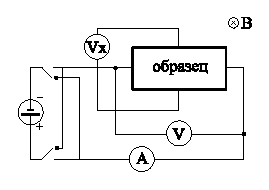
\includegraphics[height=4cm]{pic3_scheme.eps}
\caption{Линейные размеры образца и расположение основных векторов}
\label{pic3_scheme}
\end{figure}

\section{Порядок проведения работы и указания по технике безопасности}

\begin{enumerate}
\item Запустить прибор и программу для измерения эффекта Холла.
\item Выбрать схему измерения №1, активировать все блоки устройства.
\item Установить значение тока через образец равным 1 мА.
\item Провести серию измерений напряжения на образце $V$ и напряжения Холла $V_{\text{х}}$ изменяя индукцию магнитного поля от -150 до 150 мТл.
\item Повторить измерения при токе через образец равном 2 мА.
\end{enumerate}

Электрический ток в схеме не превышает 10 мА. При выполении работы действует стандартная техника безопасности при работе с компьютером.

\section{Обработка результатов эксперимента}

\begin{enumerate}
\item Результаты измерений занести в таблицу. Значения для положительных и отрицательных величин индукции магнитного поля вносятся в одну строку с указанием полярности.
\item Определить тангенс угла Холла из соотношения (\ref{eq3_tg}).
\item Определить тип и подвижность основных носителей заряда, пользуясь выражением (\ref{eq3_mu}).
\item Используя (\ref{eq3_mu}) найти коэффициент Холла, считая основным механизмом рассеяние на ионах примеси.
\item Определить погрешность измерения.
\end{enumerate}

\begin{table}[h!]
\caption{Измерение величины эффекта Холла}
\begin{center}
\begin{tabular}{c|c|c|c|c|c}
№ & I & $V_{B^{+}}$ & $V_{B^{-}}$ & $\overline{V}$ & $R_{\text{х}}$ \\
\hline
& мА & В & B & B & $\text{см}^{-3}\text{Кл}^{-1}$ \\
\hline
\end{tabular}
\end{center}
\end{table}

\section{Контрольные вопросы}

\begin{enumerate}
\item Каков механизм возникновения эффекта Холла?
\item Какие электрофизические свойства полупроводников можно исследовать с помощью эффекта Холла?
\item Как связаны коэффициенты Холла и концентрация носителей заряда в случае примесной и собственной проводимости?
\item Отклонение электронов и дырок под действием силы Лоренца.
\item Критерии слабых и сильных электрических и магнитных полей.
\item Дрейфовая и холловская подвижность свободных носителей заряда.
\item Определение Холл-фактора, его зависимость от степени вырождения и механизма рассеяния в полупроводнике.
\item Природа возникновения паразитных ЭДС, возникающих при исследовании эффекта Холла.
\item Как определить доминирующий механизм рассеяния носителей заряда?
\item Эффект Холла в полупроводнике со смешаным типом носителей заряда.
\end{enumerate}

\section{Литература}
\begin{enumerate}
\item П.С. Киреев. Физик полупроводников. М.: Высшая школа, 1975.
\item Шалимова К.В. Физика полупроводников. СПб.: Лань 2011. 416 с.
\item Абрамов В.Б., Аверин И.А., Карпанин О.В. и др. Исследование свойств полупроводников методом эффекта Холла. Методические указания. Пенза. ПГУ. 2010.
\end{enumerate}
\newpage

\anonchapter{Лабораторная работа №4}
\setcounter{chapter}{4}

\begin{center}
Определение времени жизни неосновных носителей заряда по спаду фотопроводимости\\
(4 часа)
\end{center}

\section{Цель работы}
Определение рекомбинационного времени жизни в непрямозонных полупроводниках по спаду фотопроводимости бесконтактным СВЧ методом.

\section{Теоретическая часть}

\subsection{Генерация и рекомбинация}
При освещении полупроводника светом с энергией, превышающей ширину запрещённой зоны, или при протекании тока через неоднородный полупроводник, в нём могут появляться неравновесные или избыточные носители заряда. По аналогии с равновесной концентрацией носителей, имеющей место в стационарном состоянии, концентрация в данном случае носит название неравновесной. Её можно записать как:

\begin{equation}
n = n_{0} + \Delta n
\end{equation}
где $n_{0}$ - равновесная концентрация, $\Delta n$ - концентрация избыточных носителей заряда.

Изменение концентрации под освещением называется оптической генерацией. Если концентрация избыточных носителей мала по сравнению с равновесной, говорят о низком уровне генерации (или низком уровне инжекции, если речь идёт об инжекции носителей из контакта). Уровень генерации можно расчитать по закону Бугера-Ламберта. Для света интенсивности $I$ и образца с толщиной, превышающей величину $\frac{1}{\alpha}$, где $\alpha$ - коэффициент поглощения света, можно записать:

\begin{equation}
G(x) = -\frac{d I(x)}{d x} = \alpha I(x) = I_{0} (1-R) \exp(-\alpha x)
\end{equation}
где $R$ - коэффициент отражения.

Для тонких образцов стоит учитывать многократное отражение:

\begin{equation}
G(x) = I_{0} \frac{1-R}{1-R^{2} \exp(-2 \alpha d)} \exp(-\alpha x)
\end{equation}

Процесс исчезновения пары избыточных носителей при взаимодействии называется рекомбинацией.

Рекомбинация в объёме полупроводника может протекать по трём основным механизмам.

\begin{enumerate}
\item Межзонная рекомбинация - это переход электронов из зоны проводимости в валентную зону. Такой переход сопровождается испусканием энергии, которая в прямозонных полупроводниках излучается в виде света. Поэтому такую рекомбинацию называют излучательной. В непрямозонных материалах, таких как кремний и германий, излучательная рекомбинация не наблюдается, а коэффициент межзонной рекомбинации очень мал.
\item Рекомбинация через локальные центры или рекомбинация Шоккли-Рида-Холла - это процесс, при котором электроны переходят из зоны проводимости на разрешённые уровни в запрещённой зоне (их роль обычно играют атомы примеси и дефекты решётки), а уже с них - в валентную зону.
\item Оже-рекомбинация - это процесс, при котором электрон, переходя в валентную зону, отдаёт часть своей энергии другому электрону в зоне проводимости, благодаря чему тот переходит на более высокий уровень внутри зоны.
\end{enumerate}

Для монокристаллического кремния доминирующим механизмом является рекомбинация Шоккли-Рида-Холла.

Рассмотрим полупроводник n-типа. При низком уровне инжекции один и тот же примесный центр будет либо заполнен электронами (в электронном материале, либо дырками (в дырочном материале). Тогда при рекомбинации пары в n–типе сначала должна быть захвачена дырка из валентной зоны (электрон с центра уходит в валентную зону), затем на это место захватывается электрон из зоны проводимости. Время жизни определяется скоростью захвата дырки на примесный центр, то есть, временем жизни дырки. Поэтому в случае малого уровня инжекции говорят о времени жизни неосновных носителей заряда, хотя оно по-прежнему характеризует время жизни избыточной электронно-дырочной пары.

Скорость генерации и рекомбинации носителей характеризуется приращением концентрации в единицу времени. Процесс изменения концентрации со временем описывается уравнением непрерывности:
\begin{equation}
\frac{\partial n}{\partial t} = G_{n} - R_{n} + \frac{1}{e} \operatorname{div} j
\end{equation}

В стационарном состоянии при отсутствии градиента концентрации тепловая генерация и рекомбинация полностью уравновешивают друг друга: $G_{0} = R_{0}$. В то же время изменение внешних условий приводит к изменению уровня генерации: $G = G_{0} + \Delta G$. При этом изменяется концентрация избыточных носителей $n = n_{0} + \Delta n$. Рекомбинация, как в равновесном, так и в неравновесном случае характеризуется одинаковой величиной $\omega$, равной вероятности рекомбинации одного носителя за единицу времени. Полное число носителей, прорекомбинировавших за единицу времени, таким образом, составит $R = \omega n$. Вероятность имеет размерность обратного времени, поэтому можно ввести характерную величину, называемую временем жизни $\tau = \frac{1}{\omega}$. Тогда

\begin{equation}
\frac{\partial n}{\partial t} = G_{n} - R_{n} = G_{0} + \Delta G - \frac{n_{0} + \Delta n}{\tau} = \Delta G - \frac{\Delta n}{\tau}
\label{eq4_contin}
\end{equation}

Если величина $\tau$ не зависит от концентрации носителей, то есть, не меняется со временем, то она численно равно времени, за которое избыточная концентрация неравновесных носителей спадает в $e$ раз ($e = 2.72$):

\begin{equation}
\Delta n(t) = \Delta n_{0} \exp \left( -\frac{t}{\tau} \right)
\end{equation}
что является точным решением дифференциального уравнения (\ref{eq4_contin}) при условии $\Delta G = 0$.

В общем случае $\tau$ может зависеть от величины избыточной концентрации или уровня инжекции. В таком случае из (\ref{eq4_contin}) выводится понятие мгновенного времени жизни, которое есть отношение избыточной концентрации неравновесных носителей к скорости изменения этой концентрации из-за рекомбинации в объёме:

\begin{equation}
\tau = -\frac{\Delta n}{\partial n / \partial t}
\end{equation}

В одном образце рекомбинация может протекать через различные механизмы, каждый из которых характеризуется своей вероятностью $\omega_{i}$. В таком случае общая вероятность рекомбинации одной частицы равна сумме вероятностей для каждого механизма:

\begin{equation}
\omega = \sum\limits_{i} {\omega_{i}} \rightarrow \frac{1}{\tau} = \sum\limits_{i} {\frac{1}{\tau_{i}}}
\end{equation}

Если $\tau$ не зависит от концентрации, его можно определить по спаду фотопроводимости, то есть, по изменению со временем добавочной части электропроводности, возникающей при облучении образца светом. Стандарт ГОСТ рекомендует для этого определять время, за которое избыточная фотопроводимость спадает в $e$ раз после выключения освещения. Также существуют стационарные методы измерения времени жизни, в которых $\tau$ моно определить по абсолютной величине фотопроводимости, если известна скорость генерации: $\tau = \frac{\Delta \sigma_{max}}{e G \mu}$.

\subsection{Скорость поверхностной рекомбинации и эффективное время жизни}

В идеальном случае сигнал релаксации неравновесной концентрации носителей заряда описывается экспоненциальной функцией с параметром $\tau$. Однако образцы для измерения имеют конечные размеры. Через поверхностные состояния идут дополнительные к объемным процессы рекомбинации, что уменьшает величину измеряемого или эффективного времени жизни $\tau_{eff}$ и искажает форму релаксационной кривой. Рекомбинация на поверхности характеризуется скоростью поверхностной рекомбинации $S$, которая зависит от обработки поверхности. Для пассивированных пластин монокристаллического кремния эта скорость не превышает десятков см/с, для шлифованных образцов может превышать десятки тысяч см/с. Учёт поверхностной рекомбинации позволяет записать граничные условия для образца толщиной $2 a$ как:

\begin{equation}
D_{p} \frac{\partial n}{\partial x} = \pm s \Delta n
\end{equation}

Для описания релаксационной кривой необходимо решать уравнение непрерывности (\ref{eq4_contin}) при отсутствии генерации в объёме, но с учётом потока зарядов. Пусть пластина имеет n-тип проводимости. Будем считать, что центры прилипания отсутствуют, а уровень генерации низкий. Избыточные носители созданы импульсом света. Тогда уравнение непрерывности в одномерном случае будет иметь вид:

\begin{equation}
\frac{\partial n}{\partial t} = -\frac{\Delta n}{\tau} + \mu_{p} E \frac{\partial n}{\partial x} + D_{p} \frac{\partial^2 n}{\partial x^2}
\label{eq4_relaxation}
\end{equation}
где $D_{p}$ - коэффициент диффузии дырок, $E$ - поле, возникающее из-за градиента заряда.

Считая внутреннее поле $E$ малым, решение уравнения (\ref{eq4_relaxation}) можно записать как

\begin{equation}
\Delta n(x,t) = G \cos(A x) \exp \left( -t \left[ \frac{1}{\tau_{p}} + D_{p} \frac{\xi^2}{a^2} \right] \right)
\end{equation}
где $\xi$ - корень трансцендентного уравнения $\frac{D_{p}}{a S} \xi = \ctg \xi$.

Трансцендентное уравнение, определяющее $\xi$ имеет первое решение в интервале $\left( 0, \frac{\pi}{2} \right)$, второе решение - в интервале $\left( \pi, \frac{3 \pi}{2} \right)$ и т.д. При этом существует два точных решения этого уравнения в области $\left( 0, \frac{\pi}{2} \right)$, расположенных в крайних точках. Если $S \rightarrow 0$ то $\xi_{1} \rightarrow 0$, а если $S \rightarrow \infty$ то $\xi_{1} \rightarrow \frac{\pi}{2}$. Первый случай реализуется при измерении тонких (менее 100 мкм) пластин. В этом случае

\begin{equation}
\frac{1}{\tau_{eff}} = \frac{1}{\tau} + \frac{2 S}{d}
\end{equation}

Второй случай реализуется в образцах с непассивированной поверхностью

\begin{equation}
\frac{1}{\tau_{eff}} = \frac{1}{\tau} + \frac{\pi^2 D}{d^2}
\end{equation}

В общем случае для расчёта времени жизни можно использовать сумму этих двух решений:

\begin{equation}
\frac{1}{\tau_{eff}} = \frac{1}{\tau} + \frac{1}{\frac{d^2}{\pi^2 D} + \frac{d}{2 S}}
\label{eq4_pavelka}
\end{equation}

\section{Методика измерения и описание установки}

Работа происходит в два этапа. На первом измеряется эффективное время жизни на установке, реализующей бесконтактный СВЧ метод. На втором проводится моделирование релаксационной кривой для определения скорости поверхностной рекомбинации.

\subsection{Работа с лабораторной установкой}

Схема установки для измерения времени жизни бесконтактным СВЧ методом по спаду фотопроводимости приведена на рисунке \ref{pic4_taumetr}.

\begin{figure}[h!]\centering
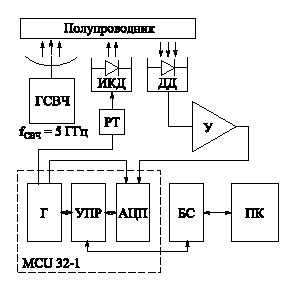
\includegraphics[height=6cm]{pic4_taumetr.eps}
\caption{Схема установки}
\label{pic4_taumetr}
\end{figure}

Генератор СВЧ излучения ГСВЧ создаёт в волноводе стоячую волну. Частота излучения 2.5 ГГц. Через кольцевой зазор в волноводе часть излучения выходит наружу и поглощается в полупроводнике. Величина поглощённой СВЧ мощности пропорциональна концентрации свободных носителей заряда. Данные об интенсивности СВЧ излучения снимаются детекторным СВЧ диодом ДД, усиливаются и отправляются в микроконтроллер.

При освещении полупроводника монохроматическим светом при помощи инфракрасного светодиода ИКД концентрация свободных носителей увеличивается. Длина волны светодиода 1.06 мкм. Прибор снимает изменение концентрации и выводит результат на экран компьютера. Длительность импульса задаётся программно. Запуск измерения производится кнопкой <<Измерить>>, файл с результатами сохраняется в памяти устройства.

Зная, что концентрация избыточных носителей изменяется по закону $\delta n(t) = \Delta n_{0} \exp(-\frac{t}{\tau})$, постоянную $\tau$ можно получить, построив график зависимости $\ln n(t)$. Котангенс угла наклона такого графика будет равен времени жизни.

Влияние поверхностной рекомбинации приводит к искажениям релаксационной кривой в начальной области. Стандарт SEMI MF-1535 рекомендует измерять время жизни по участку от 45\% до 5\% от максимального уровня выходного сигнала. Предел 5\% ограничивает уровень шума.

\subsection{Работа с программой моделирования релаксационной кривой}

Постоянная спада фотопроводимости зависит не только от свойств материала, из которого сделан образец, но и от состояния поверхности. В первом приближении формула (\ref{eq4_pavelka}) даёт близкую оценку величины рекомбинационного времени жизни в объёме полупроводника и скорости поверхностной рекомбинации. Для более точного анализа численными методами решается уравнение непрерывности. Программа расчитывает время жизни в объёме, исходя из данных о концентрации центров рекомбинации, затем строит профиль статического распределения носителей при данном уровне освещения. Затем рассчитывает скорость изменения электропроводности, анализируя изменение концентрации при рекомбинации носителей. После этого расчитывает время жизни по контангенсу угла наклона логарифма кривой спада фотопроводимости и выводит на экран полученное значение эффективного времени жизни с учётом рекомбинации на поверхности. Данные о скорости поверхностной рекомбинации, толщине образца, типе проводимости, концентрации глубоких центров и длине волны засвечивающего светодиода вводятся вручную.

В ходе работы требуется построить зависимость измеряемого времени жизни $\tau_{eff}$ от времени жизни в объёме $\tau$. Для этого на каждом шаге подбирается такая концентрация глубоких уровней $N_{t}$, чтобы $\tau$ менялось от одной микросекунды до 16 миллисекунд, увеличиваясь в два раза на каждом шаге.

\section{Порядок проведения работы и указания по технике безопасности}

\begin{enumerate}
\item Включить компьютер и установку АПК <<Тауметр>>, запустить программу для измерения времени жизни неравновесных носителей заряда.
\item Поместить образец на предметный стол установки, так чтобы образец полностью закрывал кольцевой зазор.
\item Выбрать шаг по времени так, чтобы чтобы релаксационная кривая к концу измерения интервала выходила на насыщение. Время измерения составляет 1000 шагов. Для уменьшения погрешностей проводят серию измерений с одинаковыми параметрами.
\item Выбрать ток засветки так, чтобы уровень инжекции оставался низким. Для этого сравниваются результаты измерения при разных токах лазера, и если значения отличаются более чем на 30\%, ток необходимо уменьшить по меньшей мере вдвое.
\item Расчет эффективного времени жизни производится автоматически. Нулевая точка выбирается как среднее значение последних десяти измерений, максимальная – через два шага после выключения подсветки. В окне «ГОСТ» появляется значение времени, равное моменту времени, в который максимальное значение сигнала уменьшается в 2,7 раз. В окне «ASTM» появляется значение котангенса угла наклона логарифма релаксационной кривой на участке от 45 до 5\% первоначальной интенсивности.
\item Записать результаты измерения в файл для последующей обработки.
\item Запустить программу для расчёта времени жизни.
\item Ввести толщину образца, тип проводимости, длин волны засвечивающего лазера. Сделать предположение о концентрации глубоких уровней $N_{t}$ (величина, обратно пропорциональная времени жизни в объёме полупроводника).
\item Ввести скорость поверхностной рекомбинации, исходя из предположений о пассивации образца.
\item Рассчитать профиль статического распределения, затем запустить расчёт спада фотопроводимости и расчёт времени жизни (ASTM).
\item Результаты внести в таблицу \ref{table4}.
\end{enumerate}

Электрический ток в схеме не превышает 300 мА. При выполении работы действует стандартная техника безопасности при работе с компьютером.

\begin{table}[h!]
\caption{Измерение времени жизни}
\begin{center}
\begin{tabular}{c|c|c}
№ & $\tau$ & $\tau_{eff}$ \\
\hline
& мкс & мкс \\
\hline
\end{tabular}
\end{center}
\label{table4}
\end{table}

\section{Обработка результатов эксперимента}

\begin{enumerate}
\item Из результатов измерения выделить кривую спада фотопроводимости, построить зависимость логарифма избыточной концентрации от времени, выделить линейный участок графика.
\item Меняя концентрацию глубокой примеси в образце при моделировании, построить график зависимости эффективного времени жизни от времени жизни в объёме образца для данной толщины.
\item По полученным данным определить величину времени жизни в объёме полупроводника.
\item Определить погрешность измерения времени жизни неравновесных носителей заряда.
\item Сравнить результаты измерения с формулой (\ref{eq4_pavelka}). Сделать выводы о применимости формулы для образцов данной толщины.
\end{enumerate}

\section{Контрольные вопросы}

\begin{enumerate}
\item Определение времени жизни неравновесных носителей заряда и диффузионной длины неравновесных носителей заряда.
\item Зависимость времени жизни и диффузионной длины неосновных носителей заряда от параметров материала.
\item Центры рекомбинации и прилипания неравновесных носителей заряда.
\item Диффузия и дрейф носителей в полупроводнике.
\item Нестационарные методы измерения времени жизни.
\item Влияние поверхностной рекомбинации на время жизни неравновесных носителей заряда.
\item Соотношение Эйнштейна для определения коэффициента диффузии свободных носителей заряда.
\item Влияние центров прилипания на результаты измерения времени жизни неравновесных носителей заряда.
\item Основные механизмы рекомбинации в полупроводниках.
\item Основные механизмы генерации в полупроводниках.
\end{enumerate}

\section{Литература}
\begin{enumerate}
\item В.В. Батавин, Ю.А. Концевой, Ю.В. Федорович. Измерение параметров полупроводниковых материалов и структур. М.: Радио и связь, 1985 г.
\item Л.П. Павлов. Методы определения основных параметров полупроводниковых материалов. М.: Высшая школа, 1975 г.
\item Шалимова К.В. Физика полупроводников. СПб.: Лань 2011.
\end{enumerate}
\newpage

\anonchapter{Лабораторная работа №5}
\setcounter{chapter}{5}

\begin{center}
Исследование магнетосопротивления полупроводников\\
(4 часа)
\end{center}

\section{Цель работы}
Измерение изменения сопротивления полупроводников в магнитном поле, определение дрейфовой подвижности носителей заряда.

\section{Теоретическая часть}

\subsection{Увеличение электросопротивления полупроводника в магнитном поле}

Эффект магнетосопротивления заключается в изменении электросопротивления обазца при наложении магнитного поля. Причиной возникновения этого эфекта является искривление траектории движения носителей заряда в скрещенных магнитном и электрическом полях.

\begin{figure}[h!]\centering
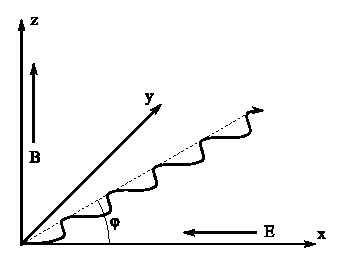
\includegraphics[height=6cm]{pic5_cycloid.eps}
\caption{Траектория электрона в скрещенных электрическом и магнитном полях внутри неограниченного полупроводника}
\label{pic5_cycloid}
\end{figure}

На движущийся заряд в магнитном поле действует сила Лоренца, которая направлена перпендикулярно дрейфовой скорости электронов $\overrightarrow{V}_{d}$ и вектору магнитной индукции $\overrightarrow{B}$. В полупроводнике заряд не может двигаться сколь угодно долго вдоль идеальной траектории, так как испытывает периодические столкновения с дефектами кристаллической решётки. При столкновении теряется энергия и, следовательно, скорость. Таким образом, носители заряда в кристалле двигаются по отрезкам циклоиды (см. рисунок \ref{pic5_cycloid}), при этом среднее направление их движения составляет с направлением поля $\overrightarrow{E}$ некоторый угол $\phi$, называемый углом Холла. Величина угла Холла определяется соотношением между дрейфовой подвижностью носителей $\mu_{d} $ и индукцией магнитного поля:

\begin{equation}
\tg \phi = \mu_{d} B
\end{equation}

Из-за того, что частица движется не по прямой, за время свободного пробега она проходит вдоль поля расстояние меньшее, чем длина свободного пробега $l_{0}$:

\begin{equation}
l_{\text{х}} = l_{0} \cos \phi
\end{equation}

В слабых магнитных полях при малом значении угла Холла

\begin{equation}
l_{\text{х}} = l_{0} \left( 1-\frac{\phi^2}{2} \right) = l_{0} \left( 1-\frac{\mu_{d}^2 B^2}{2} \right)
\end{equation}

Уменьшение пути $l_{\text{х}}$ эквивалентно уменьшению проводимости проводника:

\begin{equation}
\frac{\Delta \rho}{\rho_{0}} = \frac{\rho_{B} - \rho_{0}}{\rho_{0}} = \frac{\sigma_{0} - \sigma_{B}}{\sigma_{B}} = \frac{\l_{0} - \l_{\text{х}}}{\l_{\text{х}}} \approx \frac{\mu_{d}^2 B^2}{2}
\end{equation}

Изменение электросопротивления полупроводника пропорционально квадрату индукции магнитного поля, при этом коэффициент пропорциональности определяется величиной дрейфовой подвижности.

\subsection{Величина магнетосопротивления в ограниченном полупроводнике}

\begin{figure}[h!]\centering
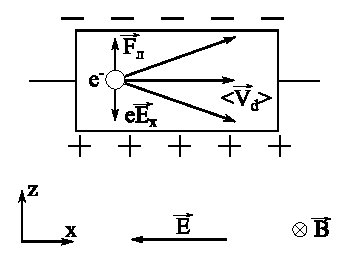
\includegraphics[height=6cm]{pic5_strip.eps}
\caption{Направления движения электронов в ограниченном образце в скрещенных электрическом и магнитном полях}
\label{pic5_strip}
\end{figure}

Рассмотрим полупроводник в виде длинного однородного стержня (рис. \ref{pic5_strip}). Под действием электрического поля $\overrightarrow{E}$ электроны движутся вдоль оси $x$. Со стороны магнитного поля $\overrightarrow{B} \perp \overrightarrow{E}$ на электроны действует сила Лоренца, направленная вдоль оси $z$. Двигаясь под действием силы Лоренца электроны скапливаются на одной из граней, заряжая её отрицательно. На противоположной грани образцется положительный заряд нескомпенсированных ионов примеси. В результате возникает поперечная ЭДС Холла, препятствующая дальнейшему разделению зарядов. Накопление зарядов будет продолжаться до тех пор, пока поле Холла не скомпенсирует отклоняющее действие магнитного поля:

\begin{equation}
e \overrightarrow{E} = -e \left[ \overrightarrow{V}_{d} \times \overrightarrow{B} \right]
\end{equation}

Если бы все электроны в кристалле имели одинаковые скорости, то они двигались бы прямолинейно вдоль оси Ox, так как кулоновская сила создаваемая полем Холла уравновешивается силой Лоренца. Однако в полупроводнике всегда имеет место некоторое распределение электронов по скоростям, обусловленное вероятностным характером рассеяния носителей. Из-за этого электроны, обладающие скоростью ниже средней будут отклоняться к одной грани образца под действием нескомпенсированного поля Холла, а обладающие более высокой скоростью - к другой, под действием нескомпенсированной силы Лоренца. При этом поток электронов в направлении приложенного поля уменьшается, что приводит к уменьшению электропроводности. За счёт того, что продольная скорость уменьшается только для электронов со скоростями, далёкими от средней, увеличение электросопротивления будет менее заментым, нежели в неограниченном образце. В вырожденных полупроводниках и металлах в проводимости участвуют прежде всего электроны, находящиеся вблизи уровня Ферми и обладающие поэтому практически одинаковыми скоростями, поэтому эффект Холла в них будет заметен гораздо меньше, чем в невырожденных полупроводниках.

Более строгий вывод эффекта магнетосопротивления может быть проведён на основе решения кинетического уравнения Больцмана. Решением являются выражения для электропроводности в присутствии магнитного поля

\begin{equation}
\sigma_{B} = e n \left< \frac{\mu}{1 + \mu^2 B^2} \right>
\end{equation}

В области слабых магнитных полей ($\mu B \ll 1$) 

\begin{equation}
\frac{\Delta \rho}{\rho_{0}} = \frac{<\mu^3>}{<\mu>} B^2 = \frac{<\mu^3>}{<\mu>^3}\mu^{2}_{d} B^2 = \frac{<\tau^3>}{<\tau>^3}\mu^{2}_{d} B^2 = C \mu^{2}_{d} B^2
\end{equation}

Величина $C$ характеризует разброс носителей по скоростям и определяется доминирующим механизмом рассеяния.

В сильном магнитном поле ($\mu B \gg 1$) 

\begin{equation}
\frac{\Delta \rho}{\rho_{0}} = \frac{<\mu>}{<\mu^{-1}>} B^2 = \frac{1}{<\mu><\mu^{-1}>} \mu_{d}^2 B^2 = \frac{1}{<\tau><\tau^{-1}>} \mu_{d}^2 B^2
\end{equation}

для ограниченного полупроводника с одним типом носителей, имеющего форму бесконечно длинного стержня, в области слабых магнитных полей ($\mu B \ll 1$) можно считать, что

\begin{equation}
\frac{\Delta \rho}{\rho_{0}} = [C - A^2] \mu^{2}_{d} B^2
\end{equation}
где $C = \frac{\left< \tau^3 \right>}{\left< \tau \right>^3}$, $A = \frac{\left< \tau^2 \right>}{\left< \tau \right>^2}$ - холл-фактор.

\subsection{Диск Корбино}
Удобной моделью неограниченного образца является диск Корбино - образец, выполненный в форме диска с отверстием в центре (рис. \ref{pic5_korbino}). Токовые контакты в таком образце расположены в центральном отверстии и по периферии диска, а магнитное поле направлено перпендикулярно плоскости диска. Линии тока наравлены от цента к краям по радиусу. Под действием магнитного поля линии тока в образце искривляются, но поперечное к электрическому поле Холла не возникает, так как не происходит разделения зарядов в образце.
\end{document}